\chapter{データセンターネットワーク}
\label{chapter:datacenter_network}
本章では, データセンターネットワークを構成する技術に関して, その概要を述べる.

\section{トポロジー}
従来のデータセンターモデルでは, HostがEdgeスイッチにつながり,
これらのスイッチがAggregationスイッチに集約され,
coreスイッチに接続するといったように, 階層的にトポロジーを形成していた~\cite{fattree}.
このような単純な階層構造を持つトポロジーは, トラフィックの大部分がデータセンター外の通信には有効であった.
しかし, 今日のようなデータセンター内で生じるトラフィックが大半を占める場合, 帯域の割当が適切でなくなる.
このような, データセンター内のトラフィックが主であれば, 階層型のトポロジーはボトルネックを引き起こす可能性がある.
近年の研究~\cite{fattree,bcube,vl2}では, トラフィックがデータセンター内に集中した時の問題を, 物理的なアプローチとして,
トポロジーを工夫する事で解消を試みている.

図\ref{fig:fattree}のように, FatTree~\cite{fattree}では, Coreスイッチを複数用いる事で,
物理パスの最大帯域を供給する.
また, 比較的狭い帯域の経路と汎用的な性能のスイッチを多数用いる.

このようなトポロジーを用いる事で, データセンター内のトラフィックに対し, 帯域を十分に使う事ができる.
しかしこのような密な配置により, 複数の経路が形成され, ルーティングをどのように決定すべきかという問題も生じる事となる~\cite{improving}.
例えば図\ref{fig:fattree}のようなFatTreeトポロジーでは, 4通りの経路が考えられる.
これら複数の経路をリンクエラー時の冗長性を持たせる目的だけでなく, 性能向上に活用することが求められている.

\begin{figure}[h]
    \begin{center}
    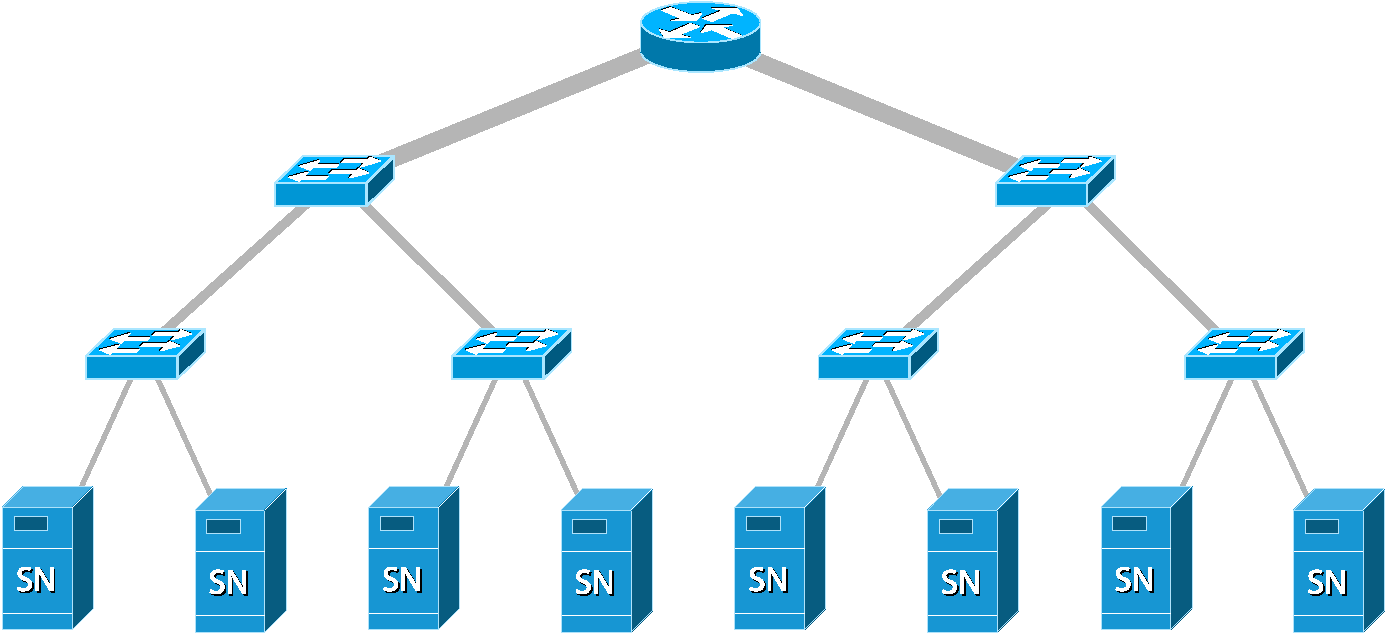
\includegraphics[autoebb, width=350pt]{./img/hierarchy_topology.pdf}
    %\caption{階層型ネットワークトポロジー}
    \caption{Hierarchical network topology}
    \label{fig:hierarchical}
    \end{center}
\end{figure}

\begin{figure}[h]
    \begin{center}
    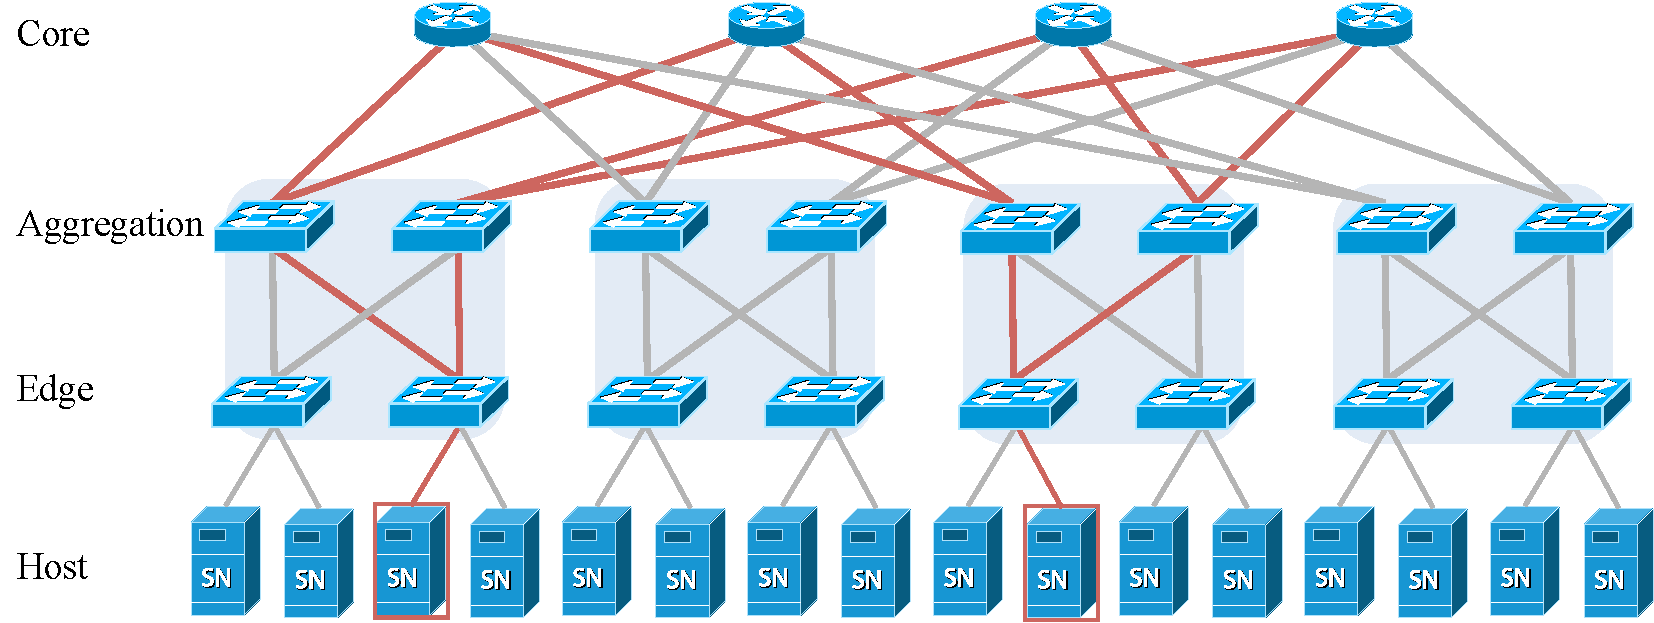
\includegraphics[autoebb, width=350pt]{./img/fattree_topology.pdf}
    %\caption{FatTreeトポロジー}
    \caption{Fattree topology}
    \label{fig:fattree}
    \end{center}
\end{figure}

\begin{figure}[h]
    \begin{center}
    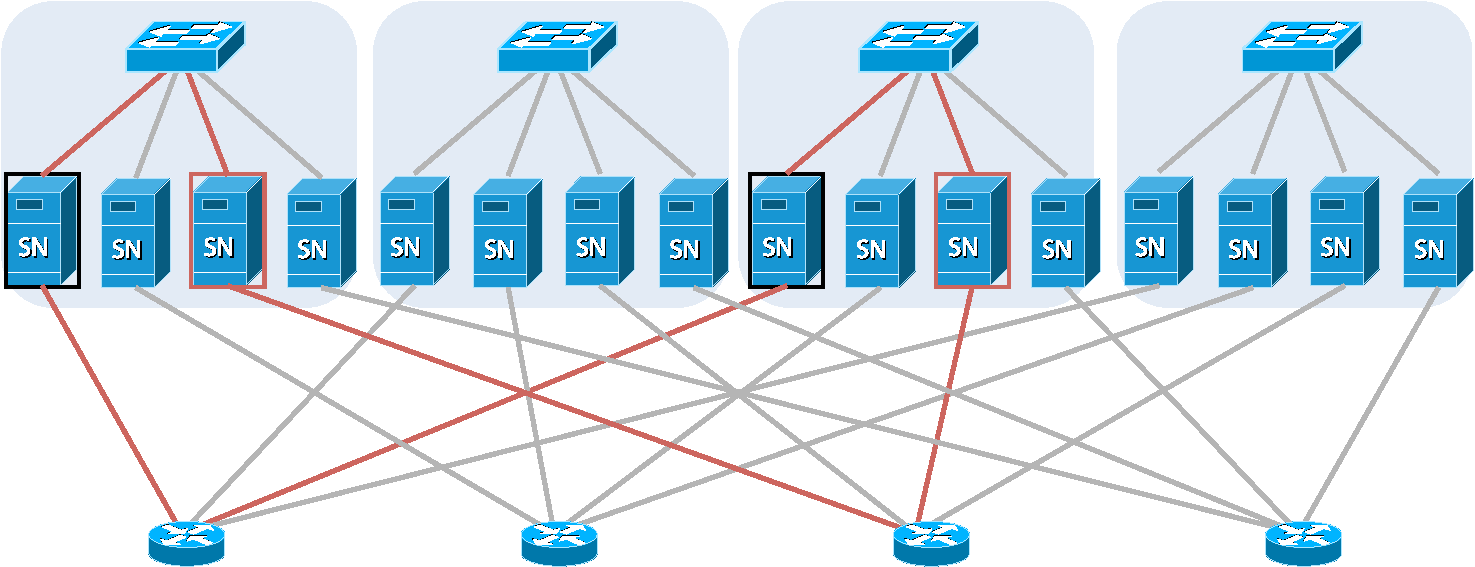
\includegraphics[autoebb, width=350pt]{./img/bcube.pdf}
    %\caption{BCubeトポロジー}
    \caption{BCube topology}
    \label{fig:bcube}
    \end{center}
\end{figure}


%
% \begin{figure}[h]
% \begin{minipage}{0.5\hsize}
% \begin{center}
% 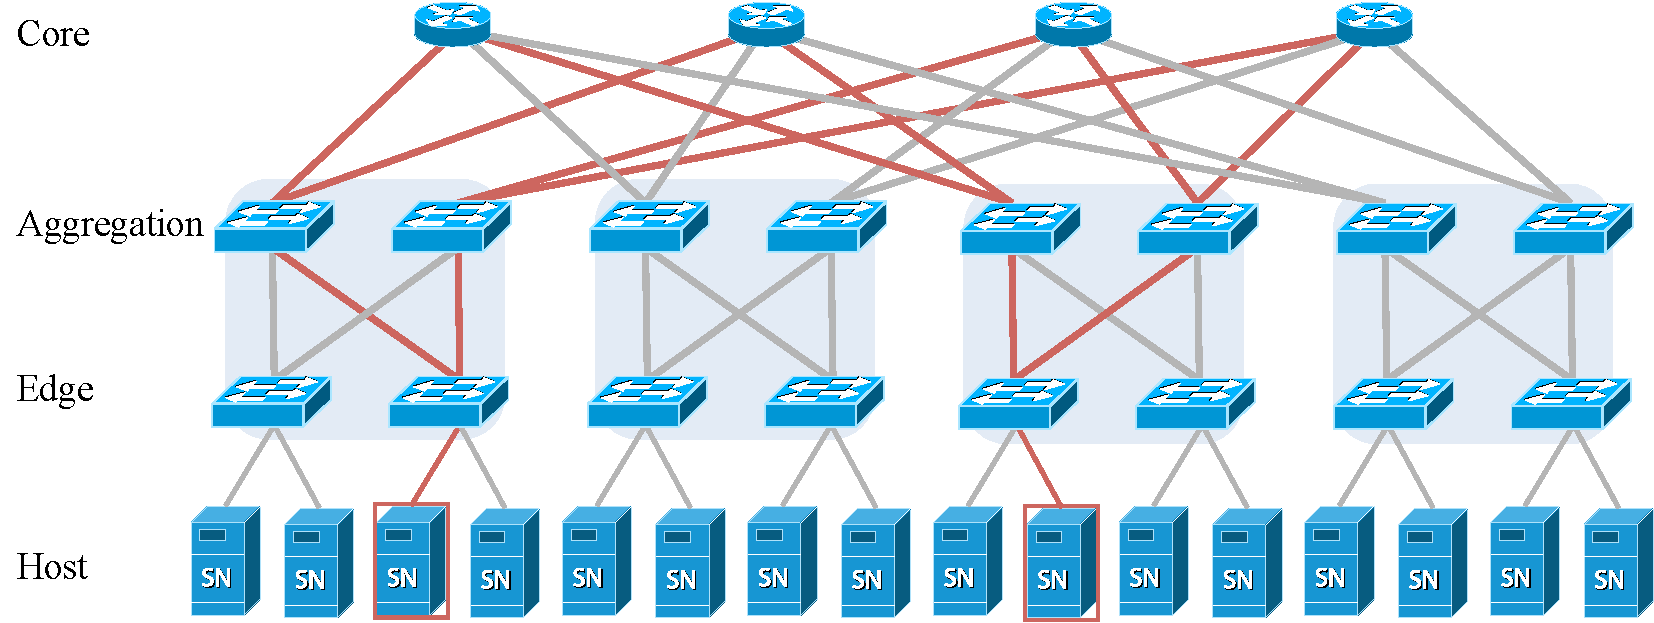
\includegraphics[autoebb, width=210pt]{./img/fattree_topology.pdf}
% \end{center}
% \caption{FatTreeトポロジー}
% \caption{Fattree topology}
% \label{fig:fattree}
% \end{minipage}
% \begin{minipage}{0.5\hsize}
% \begin{center}
% 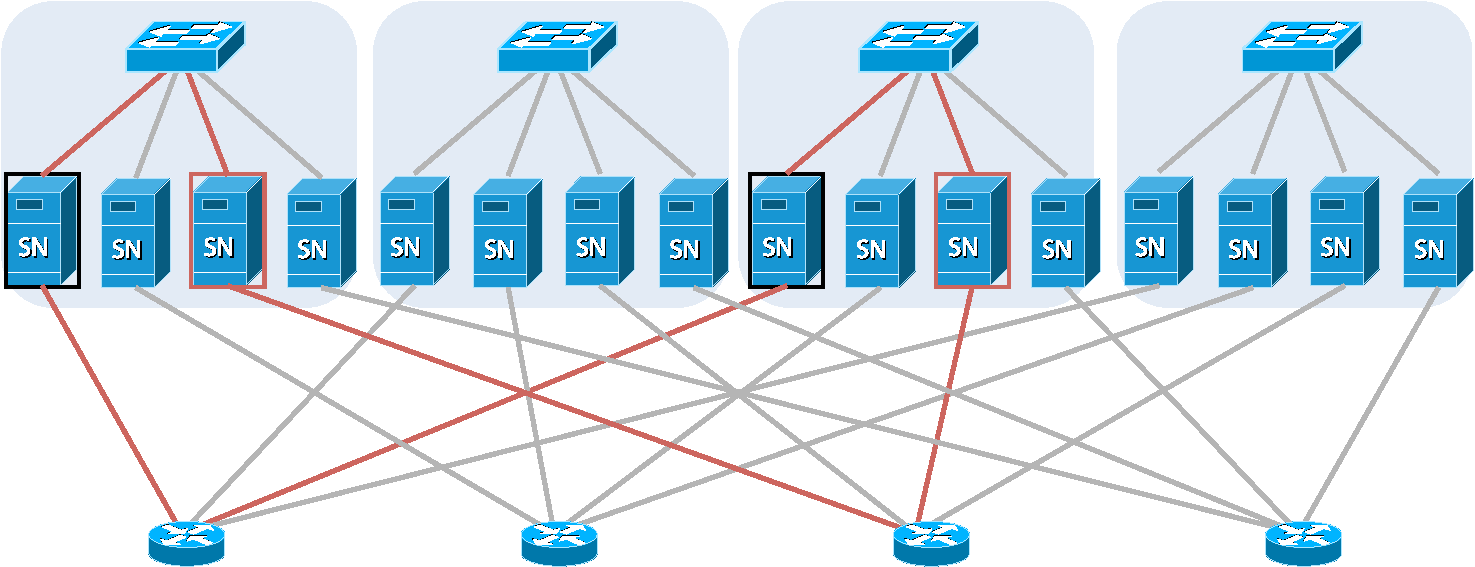
\includegraphics[autoebb, width=110pt]{./img/bcube.pdf}
% \end{center}
% \caption{BCubeトポロジー}
% \caption{BCube topology}
% \label{fig:bcube}
% \end{minipage}
% \end{figure}

\section{マルチパス, マルチホーミングを実現するプロトコル}
本節では, 複数の経路を持つデータセンター環境においてネットワーク資源の有効活用を実現するプロトコルについて述べる. 
\subsection{データリンク層におけるアプローチ}
\subsubsection{LACP}
データリンク層のプロトコルは, 通信媒体で直接接続された機器間で通信するための仕様を定めている. 
データリンク層における複数経路を利用するためのプロトコルとして, LACP(Link Aggregation Control
Protocol)がある\cite{lacp}.
LACPにより, 通信ケーブルが通信不良を起こした際にも, 束ねた回線のうち正常に動作しているケーブルによって冗長化することができる. 
また, 同一スイッチの異なる複数のインタフェースと接続し, 複数の物理リンクを束ねて,
一つの論理リンクとして扱うことで, リンク容量を集約することができる. 
LACPは, パケットヘッダーに対するハッシュ計算での物理リンクへのパケット多重化によって, 負荷分散を実現する. 
このように, LACPによって容易に帯域を拡張し, 通信性能を向上させることができる. 
データリンク層での負荷分散では, ハッシュ計算のアルゴリズムとして主にMacアドレス, IPアドレス, ポート番号などを用いるが, どの値をキーにするかは,
各ネットワーク機器の実装に依存する. 
実際, MACアドレスを用いて通信を行う際, 二つ目以降のMACアドレスを取得するすることはARPプロトコルの実装上できない\cite{arp}. 
そのためクライアントサーバ通信において, 異なる種類のスイッチによって異なるキー値をLACPの負荷分散アルゴリズムを用いる場合, 完全な負荷分散が実現できず,
通信性能の向上が見込めない.
完全な負荷分散を実現するためにはキー値を同一になるように調整する必要があるが, 現実的には困難である\cite{lacp_problem}.

\subsection{トランスポート層におけるアプローチ}

\subsubsection{SCTP}
SCTP\cite{sctp}とはTCPと同様にパケットの到達, またその到着順序を保証する信頼性のあるプロトコルであり,
標準でマルチホーム機能をサポートしている.
標準化されているプロトコルにおいてマルチホーム機能は冗長性のためのものであり, 冗長経路へ新しいデータを送信することは推奨されていなかった. 
そこでSCTPにおいて, 冗長回線を用いた帯域集約を行うプロトコルであるCMT (Concurrent Multipath
Transfer)が提案された\cite{cmt_1, cmt_2}. 
CMTでは, 期待されていた値よりもウィンドウサイズが増加しないという課題があり, 大きく3つの欠点に対して改善が行われた.  

\begin{description}
 \item[送信者による不要な再送処理]\mbox{}\\ 
        SACKパケットのパケット損失情報とそれぞれのパケットの宛先アドレスから, パケットロスなのか順序の入れ替えなのかを判断し,
        最小限での再送制御を実現している. 
 \item[送信者側におけるウィンドウサイズの更新頻度の少なさによるウィンドウサイズの増加の抑制]\mbox{}
        新しいパケットに対するACKパケットのみに従いウィンドウサイズを更新していたため, ウィンドウサイズ増加が抑制された. 
        CMTではパケットをどの宛先に送信したかを把握しておくことで, 回線に応じたウィンドウサイズの増加を行うようにした. 
 \item[ACKパケットの増加]\mbox{}\\
        SCTPやTCPにおいてパケットが順序通りに受信できた場合に,
        遅延ACKによって複数のACK応答を一つにまとめることで通信オーバーヘッドを減らしていたが,
        CMTでは複数回線を集約しているためパケットが順序通りに届かないことが多くACKパケットが増加していた. 
        そこで, CMTでは順序通りに届かない場合においてでも, ACKの送信を遅らせることにより, ACKのオーバーヘッドを削減した. 
\end{description}
SCTPを拡張したマルチパス通信のメリットはSCTP自体にマルチホーム機能をサポートしていることにある. 
しかし, SCTPは現在様々な通信において広く利用されているTCPやUDPとは異なるプロトコルであるために,
既存のアプリケーションに対して変更が生じるという課題がある. 


\subsubsection{Multipath TCP}
MPTCPは, 一つの経路でデータ転送するTCPを拡張し, 複数のインタフェース,
あるいは複数のポートを用いてデータ転送をするプロトコルである~\cite{mptcp}.
クライアントが複数のIPアドレスを持っていた場合, 新たにサブフロー\footnote{複数のTCPコネクションの内,
ある一つのコネクションにおけるフロー}のコネクションが確立される.
追加されたサブフローは, クライアントの持つインターフェースが1つの場合, 同じIPアドレスで異なる送受信ポートを用いる.
インターフェースを複数持つ場合には, 異なるIPアドレスの組み合わせで通信を行う.
ルーティングに関しては, 複数の宛先IPアドレス, 送信元アドレスからそれぞれ経路決定される.
このように, アプリケーション層より下のレイヤーのみで複数の経路を使ってデータ転送を行うため,
アプリケーション側がMPTCPでの通信を意識することなくデータ転送ができる.

MPTCPでは, サブフローが, それぞれのシーケンス領域を持ち, 経路状態に合わせて輻輳制御をする~\cite{cong}.
輻輳制御には, TCPと同様にAIMD(additive-increase and
multiplicative-decrease)による輻輳制御がサブフロー単位で行われる.
以下にAIMDアルゴリズムを示す.

\begin{itemize}
\item サブフロー $r$において,
1ACKごとにウィンドウサイズ$\omega_{r}$をmin$(\frac{\alpha}{\omega_{total}},
\frac{1}{\omega_r})$増加させる.
\item サブフロー $r$において, パケットロス時にウィンドウサイズ$\omega_r$を$\frac{\omega_r}{2}$へ減少させる.
\end{itemize}
ここで, $\omega_{total}$は全てのサブフローのウィンドウサイズの総和, $\alpha$は送信速度の増加量を示すパラメータで,
以下のように定義される~\cite{cong}.

\vspace{-2mm}
\begin{eqnarray}
 \alpha = \omega_{total} \times
\frac{\displaystyle \max_{r} \frac{w_r}{RTT^2_r}}{\displaystyle
(\sum_{r}\frac{w_r}{RTT_r})^2}
\label{alpha}
\vspace{-2mm}
\end{eqnarray}

ここで, $RTT_r$はサブフロー$r$でのラウンドトリップ時間を示している.
MPTCPでの輻輳制御には二つの性質ある.
一つは, サブフローのウィンドウサイズは, 全てのウィンドウサイズの大きさに依存するということである.
これにより, 混雑したサブリンクにおいては, ウィンドウサイズが抑えられ, ロードバランスができる.
二つ目は,MPTCPのアルゴリズムによって, TCPでの輻輳制御よりも悪化する事を回避している事である.
しかし, もし複数のサブフローがそれぞれ混雑のないサブリンクを利用する場合, いずれかのコネクションが帯域を占有する可能性がある.


\section{トラフィック}
\label{sec:traffic}

大量の計算機資源を有効活用するためには,
並列分散処理フレームワークを用いられ, 多数の処理ノードと分散処理の制御をする管理ノードから構成されているpartition-aggregate構造をとり,
管理ノードからクエリーが発行され, 処理ノードがそれを受け取り,レスポンスを返す.
このとき, トラフィックパターンが  (1){\it Query traffic}, (2){\it Short message
traffic}, (3){\it Backgroung traffic}の3つに分類される~\cite{dctcp}.

{\bf Query traffic. }Query trafficとは, 大規模計算処理を分割して並列処理を開始する際に,
aggregatorノードから処理ノードへ具体的な処理を割り当てるためのトラフィックである.
Query trafficの特徴は, 非常に小さいフローサイズ(2KB$\sim$20KB)で,
フローの役割上, 処理全体の遅延に非常に強く影響を及ぼす事である.
そのため, アプリケーション性能を考慮すると, 低レイテンシでの通信が求められている.
また並列分散処理システムの構成上, Query trafficはms$\sim \mu$s単位で生成され,
バースト性があるといえる~\cite{dctcp}.

{\bf Short message traffic. } Short message trafficとは,
処理ノードの動作を制御するためのトラフィックである.
Short message trafficの特徴は, フローサイズは50KB$\sim$1MBで, Query
trafficと同様に処理全体の遅延に影響を及ぼすという事である.
しかし, Querry trafficほどのフロー数は生成されず, 生成間隔も秒単位である.

{\bf Backgroung traffic. }Backgroung trafficは,
各処理ノードへ更新データを送信するトラフィックである.
Backgroung trafficの特徴は,フローサイズが1MB$\sim$50MBと大きいことにある.
さらに, その生成間隔は大きい.
また, Backgroung trafficでの更新データは, 処理精度の向上に寄与するが, 処理に必須ではないので,
処理全体の遅延にはつながらない.

つまり, 分散処理開始時に生成されるQuery trafficが遅延すると,
処理全体に対し遅延を引き起こすので, Query trafficを含むショートフローのフロー完結時間は極めて重要なメトリックである.

また, Alizadehらは, 実際のデータセンターのトラフィックでは, レイテンシ志向なショートフローとスループット志向なロングフロー,
そしてバースト性のあるQuery trafficが混在していると報告している.
さらに, Background trafficのフロー数自体は少ないが,
全体のトラフィック量の大部分がBackgroung trafficによって占められているという特徴がある~\cite{traffic}.

フローがデッドライン時間までに完結するためには, フローのサイズも大きく影響がある. 
つまり, 事前に通信が発生するフローサイズを知っておくことが重要である. 
実際, 今日の大部分のクエリーレスポンスアプリケーションにおいては, 処理ノード同士のフローのサイズは通信開始時に決定する. 
例えばウェブ検索アプリケーションでは, top-k queryアルゴリズムなどを用いて, 基本的には上位k件の結果のような固定的なレスポンスを返す. 
キーバリューストア\cite{key-value1, key-value2}や並列分散処理\cite{mapreduce,
dryad}などの技術でも同様である.  
従って, 多くのウェブアプリケーションにおいて, 実際に処理が終わった後ではなく, 通信が開始した時点で, 
アプリケーションのコードからレスポンスフローのサイズを知ることができる.


\section{アプリケーション}
今日の主なデータセンターアプリケーションとしてOLDI(OnLine Data Intensive)アプリケーションがあり,
``オンライン性''と``集約性''の大きく2種類の特徴がある\cite{oldi}.
``オンライン性''とはクライアントとサーバーとのインタラクティブな通信を示している. 
具体的には, クライアント側からブラウザ経由でクエリーを送り, サーバ側はクエリーを受けるとすぐにレスポンスを返す通信を行う. 
OLDIアプリケーションでは, 一つの通信に対して例えば300ms以内のようにデッドラインを超えないようにレスポンスを返すことが期待されている. 
一方``集約性''とは, 大量のデータからレスポンスを生成することを示している. 
具体的には, Webサーチのような全文検索により結果を返すような演算のことである. 
実際のデータセンターでは, 大規模なデータセットは数千台規模のサーバに分散して格納されており,
クエリーに対して対象のデータが格納されているサーバーに対して検索を行う. 

こうした二つの特徴を持ったOLDIアプリケーションはFig.\ref{fig:oldi_tree}に示すようなツリー型のアーキテクチャによって構成され,
partition-aggregation型アルゴリズムによって処理が行われる. 
このような構成を取るため, 上記のような性質が性能の面で問題になる.\cite{websearch} 
Fig.\ref{fig:oldi_tree}ではアーキテクチャは二段によって構成されているが,
アプリケーションの規模によってはより深いツリーとなることもある. 
partition-aggregation型アルゴリズムでは, まずrootノードがクライアント側から送られてきたクエリーを受けとり,
クエリーの対象データが格納されているWorkerノードへとジョブが分割される. 
それぞれのWorkerノードがレスポンスを返し, Aggregatorノードはそれらを集約する. 
さらに, RootノードがそれぞれのAggregatorノードのレスポンスを集約し, 最終結果をクライアントへ返す. 
Rootノードから各Workerノードへのクエリーの下り通信と, 各WorkerノードからRootノードへのレスポンスの上り通信は,
アプリケーション性能の観点から, デッドライン時間以内に完結されるべきである. 
それぞれのデッドライン時間は, アプリケーションが満たすべきデッドラインから, そのアプリケーションが構成しているアーキテクチャの段数によって割り当てられる. 
例えばFig.\ref{fig:oldi_tree}では,
Workerノードはクエリーを受け取ってから30ms以内にAggregatorノードへレスポンスを返さなければならない. 
もし, デッドライン時間を超えてしまった場合には, Aggregatorノードは得られたレスポンスのみを集約し, Rootノードが最終的にレスポンスを返す. 
その結果, レスポンス結果の品質に影響が出ることとなる. 

それぞれのWorkerノードの演算時間は,  Workerノード自身の演算時間と, Aggregatorノードとの通信時間のそれぞれの和となっている. 
それぞれのデッドラインの決定には, 処理結果の質とレスポンス時間のトレードオフとなる. 
通信時間に対して余裕のあるデッドラインを設定した場合, デッドラインを超えるノードの数は少なくなるが, 各処理ノードでの演算かける時間が少なくなり,
十分な質の結果が出せない可能性もある. 
具体的には, 検索対象とするデータの範囲を小さくすることで処理時間を節約することとなる. 
そのため,  より多くのノードがデッドラインを超えないようにするためのデッドライン時間を設定するだけでなく,
より良い結果を返すために演算時間にも十分な割り当てが必要である.\cite{d2tcp} 

次に, Aggregatrtorノードのが各Workerノードへクエリーを送った時のAggregatorノードが構成するサブツリーでの挙動について考える. 
すべての処理ノードがほぼ同時刻にレスポンスを受け取り, 同じデッドライン時間を持っている. 
その結果, 多対1通信の大量のトラフィックがAggregatorノードへ到達する\cite{dctcp, incast}. 
そのため一つのノードへレスポンスが同期しないように,
ジッターを混ぜることでAggregatorノードのメモリーを圧迫しないようなアプリケーションレベルの工夫もされているが,
その結果テール状に遅延が発生する\cite{desynchro}.
またデータセンターでは複数のアプリケーションが同時に起動しているため,
こうしたバースト性のあるレスポンストラフィックは一つのスイッチにおいてでも同時多発的に発生すると考えられる.

さらに, こうした比較的サイズの小さい大量の多対1通信に加え,
データセンターネットワークでは長時間通信を行うバックグラウンドトラフィックも同時に通信を行っている. 
バックグラウンドトラフィックは, 各処理ノードに対して, 最新のデータを更新するための通信であり, 長時間にわたり非常に大きなデータサイズを通信する. 
それにより, 既存のTCPの性質上, こうしたロングフローがスイッチのバッファを使い果たすこととなる. 

上記のような大量の多対一トラフィックと長時間通信を行うバックグラウンドトラフィックによって, スイッチのバッファが圧迫され, 遅延が生じてしまう. 
こうした性能障害を解決するための手法の一つとして, バッファに溜まったパケットの処理高速化がある. 
実際, データセンターの一部で用いられるネットワーク機器では, 特定の用途のためにASICによるオンチップパケットバッファメモリを持つモジュールが用いられる. 
しかし, 近年のデータセンターでは汎用的なネットワーク機器を用い, コストを低くして運用する傾向があり,
特定の用途に特化した高価で複雑な構成のスイッチ機器を用いられることは多くはない.\cite{memory} 
また, バックグラウンドフローによるバッファの圧迫により大きなキューイング遅延を引き起こし,
OLDIトラフィックのデッドラインを超えるほどの遅延を引き起こすため, 
バースト性のあるトラフィックによる遅延問題を解消するためには, バックグラウンドフローに対する改善が必要である\cite{dctcp}. 

この輻輳の問題は, OLDIアプリケーションが持つ基本的な性質であるが,
今日のデータセンターネットワークではデッドラインを超えないために大きく二つの改善を行っている. 

一つは, ネットワーク機器によるスケールアウトである. 
TCP/IPネットワークでは, 基本的にパケットロスが起こった際にタイムアウト時間からエンドノードへと経路の輻輳状態がフィードバックされる. 
そのため, パケットロスが生じたときには, RTO時間の間, 新しいデータを送信することができず, デッドラインを超えてしまう. 
また, ウィンドウサイズも減少し, 通信レートも下がる. 
こうした課題対して, (1)ネットワーク帯域の増強, (2)通信時間の割り当ての増加によって, 改善する手法がある. 
前者のアプローチは比較的大きなコストがかかるが, 後者の場合, より多くの処理ノードを追加し, 一つのノードあたりの処理時間を減らすことによって,
その分通信時間への割り当てを大きくすることができる. 

もう一つは, フローに対する優先付けである. 
理想的には, デッドラインが近づいているフローに対しては優先的に通信を行い, 比較的余裕のあるフローに対しては後回しにする処理をすればよい. 
しかし, 現状広く用いられているTCPは通信の公平性を持つプロトコルであり, デッドラインによる区別は行わない. 
OLDIアプリケーションはデッドラインに依存せず, 公平にネットワーク資源を分配するが,
そのようなプロトコルがデータセンターネットワークに対して適しているとは言えない\cite{d3}. 


\begin{figure}[t]
    \begin{center}
    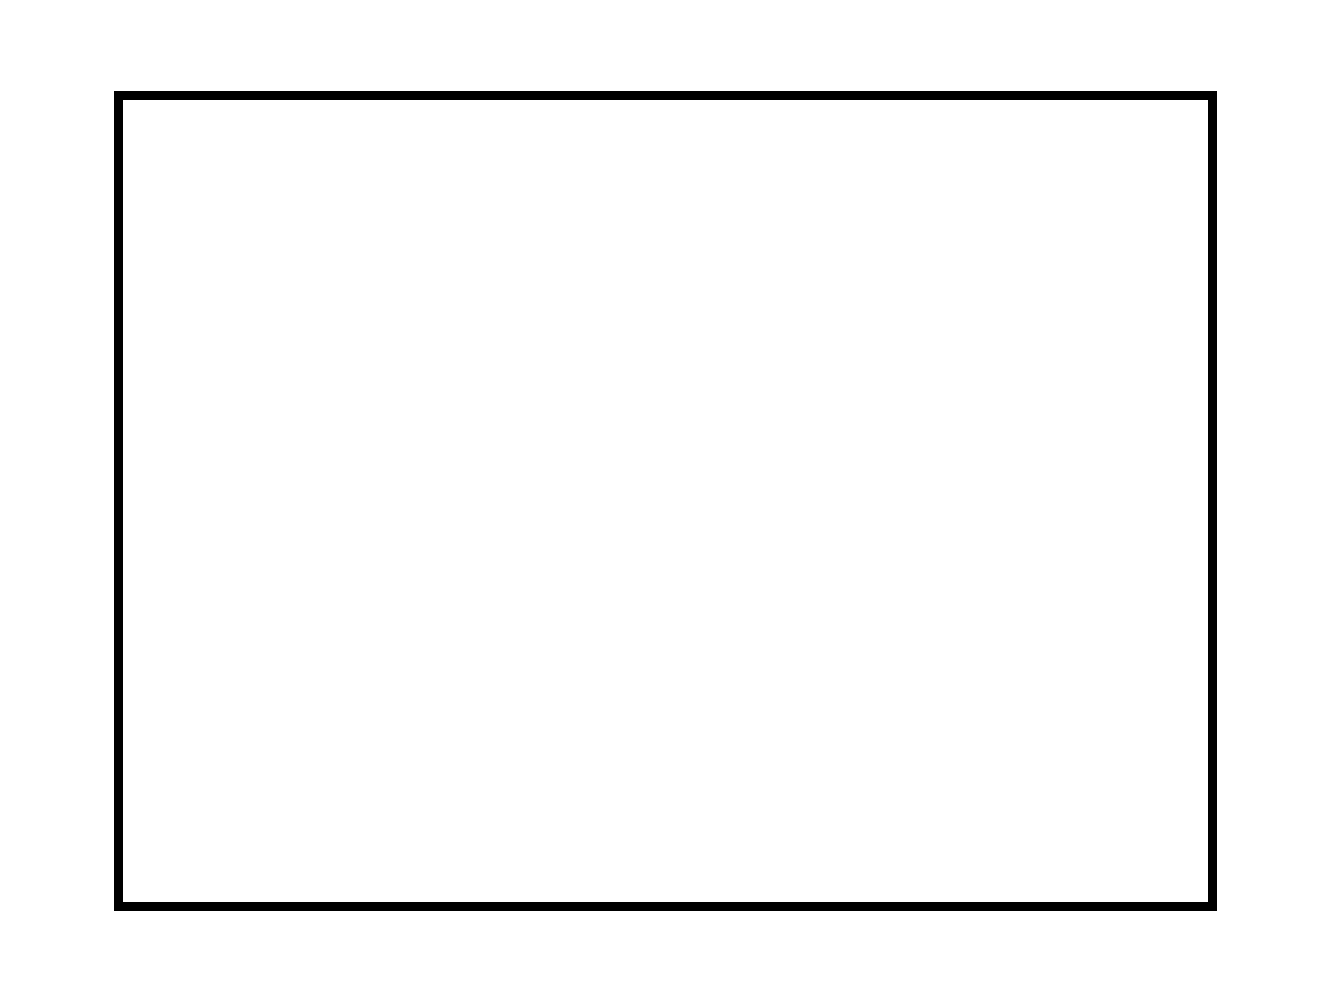
\includegraphics[autoebb, width=200pt]{./img/test.pdf}
    \caption{OLDI architecture:OLDIアプリケーションアーキテクチャ(集約の際のデッドラインも)}
    %\ecaption{The control loop in DCTCP}
    \label{fig:oldi_tree}
    \end{center}
\end{figure}